\documentclass[journal]{IEEEtran}

% Packages
\usepackage{cite}
\usepackage{amsmath,amssymb,amsfonts}
\usepackage{algorithmic}
\usepackage{graphicx}
\usepackage{textcomp}
\usepackage{xcolor}
\usepackage{booktabs}
\usepackage{multirow}

% Macros
\newcommand{\mbf}[1]{\mathbf{#1}}
\newcommand{\bs}[1]{\boldsymbol{#1}}

\begin{document}

\title{Latency-Aware Phase Optimization for Reconfigurable Intelligent Surfaces in Mobile Scenarios}

\author{Seda Savaşçı Şen%
\thanks{This work was supported by [TÜBİTAK grant number if applicable].}%
\thanks{S. Savaşçı Şen is with the Department of Electrical and Electronics Engineering, [Your University], Turkey (e-mail: sedasavascisen@gmail.com).}%
\thanks{Manuscript received [date]; revised [date].}}

\markboth{IEEE Transactions on Wireless Communications, Vol.~XX, No.~X, [Month] 2027}%
{Savaşçı Şen: Latency-Aware Phase Optimization for RIS in Mobile Scenarios}

\maketitle

\begin{abstract}
Reconfigurable intelligent surfaces (RIS) promise significant performance gains by dynamically controlling wireless propagation. However, existing work focuses on convergence quality while largely ignoring computation delay—a critical constraint when channel coherence time is finite. This paper demonstrates that latency is not secondary but a first-class design constraint fundamentally changing method rankings. Through rigorous analysis of multi-user MISO downlink with geometry-based channels, we prove three results: (1) fresh beamforming with instantaneous channel state information (CSI) outperforms stale converged phase by 11.7--14.2$\times$ at coherence time $T_c=28.2$ ms (Lemma~1); (2) an intrinsic optimum exists at $L^*\approx 8$ iterations for pedestrian mobility, with deep convergence ($L=48$) costing 5.9\% despite superior initial quality (Theorem~1); (3) per-step latency variation (2.8$\times$) causes complete ranking reversal when methods are compared under equal milliseconds rather than equal iterations (Proposition~1). All 41 claims are backed by executable scripts with sabotage-tested integrity. Results provide practical guidelines: terminate gradient descent at $L=4$--$8$ for pedestrian users, and rank methods by latency-adjusted effective rate $\rho^2(T_{\text{proc}})\cdot g(L)$, not $t=0$ quality alone.
\end{abstract}

\begin{IEEEkeywords}
Reconfigurable intelligent surface, latency-aware optimization, mobile communications, phase optimization, computation delay, channel aging, Jakes model
\end{IEEEkeywords}

%===============================================================================
% SECTION I: INTRODUCTION
%===============================================================================
% SECTION I: INTRODUCTION
% Polished with crisp contributions

\section{Introduction}
\label{sec:intro}

\IEEEPARstart{R}{econfigurable} intelligent surfaces (RIS) have emerged as a transformative technology for sixth-generation (6G) wireless networks, offering unprecedented control over the electromagnetic propagation environment through passive beamforming~\cite{Basar2019Access}. By dynamically adjusting the phase shifts of numerous low-cost reflecting elements, RIS can enhance coverage, improve spectral efficiency, and enable new applications across millimeter-wave and terahertz bands~\cite{Wu2019TWC}.

\subsection{The Latency Blind Spot in RIS Optimization}

The vast majority of RIS optimization research focuses on maximizing performance under the implicit assumption that computation time is negligible or exogenous to algorithm design. Classical approaches include alternating optimization (AO)~\cite{Wu2019TWC}, weighted minimum mean-square error (WMMSE)~\cite{Guo2020TCOM}, and projected gradient descent (PGD). Recent work has explored deep learning for direct phase prediction~\cite{Huang2020TWC,Elbir2020WCL}, motivated by the potential to bypass iterative optimization entirely.

However, these studies share a critical limitation: \textbf{they evaluate methods by convergence quality alone}, measuring performance at the endpoint of optimization without considering the time required to reach it. In static channels this evaluation is appropriate. In mobile scenarios it is fundamentally flawed.

\subsection{The Mobility-Latency Paradox}

Mobile users experience time-varying channels with finite coherence time $T_c$. At carrier frequency $f_c = 3$ GHz and pedestrian velocity $v = 1.5$ m/s, coherence time is approximately 28.2 ms~\cite{rappaport_wireless}. Any computation exceeding this duration renders the optimized phase outdated before deployment.

This creates a fundamental trade-off: \textit{converged solutions require many iterations, but by the time convergence is achieved, the channel has changed}. Classical projected gradient ascent achieves near-optimal performance with 1000 iterations but requires approximately 5600 ms---199$\times$ longer than coherence time. By the time the optimal phase is computed, it is applied to a completely different channel state.

The consequence is striking: \textbf{designing for convergence systematically misallocates computational resources}. Methods are ranked by their quality at $t=0$ (when optimization begins) rather than their quality at $t=\tau$ (when results become available), where $\tau$ is the algorithm-dependent processing delay.

\subsection{Gap in Existing Literature}

While mobility and channel aging have been studied extensively in MIMO systems~\cite{Jindal2006IT}, the interaction between \textit{computation delay} and \textit{channel aging} remains largely unexplored in the RIS literature. Existing mobility-aware RIS work~\cite{Huang2021TWC,Papazafeiropoulos2022TCOM} typically assumes zero or negligible computation time, focusing instead on tracking accuracy or channel prediction horizons. Predictive beamforming schemes~\cite{Ma2020WCL,Liu2022TCOM,Zhao2023WCL} forecast future channels $\hat{\mbf{H}}(t + T_{\text{proc}})$ but \textit{fail to eliminate staleness} because prediction itself consumes time---the cumulative delay $T_{\text{pred}} + T_{\text{opt}}$ still renders the phase configuration stale.

To our knowledge, no prior work has:
\begin{itemize}
    \item \textbf{Quantified} the value of fresh beamforming relative to stale optimized phase in RIS systems
    \item \textbf{Proven} the existence of an intrinsic optimum (finite iteration count that maximizes effective rate)
    \item \textbf{Demonstrated} that method ranking systematically reverses under equal-millisecond comparison
    \item \textbf{Provided} reproducible measurements with documented experimental scripts and sabotage-tested audit framework
\end{itemize}

\subsection{Contributions}

This paper fills this gap through rigorous latency-aware analysis of RIS phase optimization in mobile multi-user scenarios. Our main contributions are:

\begin{enumerate}
    \item \textbf{We prove fresh beamforming dominates stale optimized phase} (Lemma~\ref{lem:fresh_dominance}): Fresh beamforming with instantaneous CSI is 11.7--14.2$\times$ more valuable than stale converged phase at coherence time $T_c = 28.2$ ms. This corrects a previously reported but non-reproducible claim of ``17$\times$ gain'' for which no executable script existed. Our measurement is fully reproducible via scripts/mumiso\_beam\_staleness.py with 10{,}000 independent channel realizations.

    \item \textbf{We prove the existence of an intrinsic optimum at finite iteration count} (Theorem~\ref{thm:intrinsic_optimum}): We identify $L^* \approx 8$ gradient steps as the intrinsic optimum for pedestrian scenarios ($v = 1.5$ m/s, $f_c = 3$ GHz), achieving 5.380 bps/Hz effective rate. Designing for deep convergence ($L=48$ steps) costs 5.9\% in achievable rate despite superior t=0 performance, proving that \textit{mathematical convergence is not physically optimal} under mobility.

    \item \textbf{We prove method ranking systematically reverses under equal-millisecond constraints} (Proposition~\ref{prop:ranking_reversal}): Per-step latency variation (2.8$\times$ between learned updates and Adam optimizer) causes \textit{complete ranking reversal}. Under equal-iteration comparison, learned gradient updates win at all five budgets ($L=1,2,4,8,16$) with 68.3--83.7\% win rates. Under equal-millisecond comparison, all five learned configurations are dominated by classical Adam optimizer across five independent trials, confirming that per-iteration latency is a first-class design constraint.

    \item \textbf{We provide a reproducibility framework with sabotage-tested integrity}: All 41 audited claims are backed by executable scripts in a version-controlled repository. Sabotage testing (writing untrained weights to trained checkpoints) caused 7 out of 41 assertions to fail, confirming the audit measures genuine model quality rather than cached constants. We document measurement traps (machine load contamination, timing jitter, prefix non-stability) that affect latency-dependent conclusions, and provide idle-machine validation protocols to prevent contamination.
\end{enumerate}

\subsection{Paper Organization}

Section~\ref{sec:related_work} positions our work relative to classical optimization, deep learning, mobility-aware design, and predictive beamforming literature. Section~\ref{sec:system} presents the 3GPP-compliant system model, Jakes mobility framework, and latency-aware effective rate formulation. Section~\ref{sec:analysis} establishes the theoretical foundation through three main results (Lemma~\ref{lem:fresh_dominance}, Theorem~\ref{thm:intrinsic_optimum}, Proposition~\ref{prop:ranking_reversal}). Section~\ref{sec:measurements} describes the reproducibility framework and measurement protocols. Section~\ref{sec:results} validates the theoretical findings through extensive simulations. Section~\ref{sec:conclusion} concludes the paper and discusses future directions.


%===============================================================================
% SECTION II: RELATED WORK
%===============================================================================
\section{Related Work}
\label{sec:related_work}

\subsection{RIS Phase Optimization}
Joint precoding and RIS phase design has been addressed with alternating optimization and semidefinite relaxation~\cite{Wu2019TWC}, beamforming under practical phase-dependent amplitude models~\cite{Abeywickrama2020TCOM}, block-coordinate-descent designs for multicell systems~\cite{Pan2020TWC}, fractional programming for weighted sum-rate maximization~\cite{Guo2020TWC} and fixed-point and manifold optimization~\cite{Yu2019ICCC}, and WMMSE-based rate maximization~\cite{Choi2024TCOM} building on the WMMSE algorithm~\cite{Shi2011TSP}. These methods are evaluated by the objective value they reach; their run time, when discussed, is characterized by complexity order rather than by measured latency relative to the channel's coherence time.

Learning-based designs replace the iterative solver with a trained policy, for example deep reinforcement learning for joint precoding and phase design in multi-user MISO systems~\cite{Huang2020JSAC}, or learning to reflect and beamform directly from received pilots without explicit channel estimation~\cite{Jiang2021JSAC}. Algorithm unrolling, which turns the iterations of an optimizer into the layers of a trainable network~\cite{Monga2021SPM}, is the template for the learned update rule studied here; it has been applied to IRS beamforming to avoid the cost of matrix inversions in an iterative solver~\cite{Liu2022TWC}; it has also been used for MIMO detection~\cite{Samuel2019TSP} and for WMMSE precoding~\cite{Hu2021TWC,Pellaco2022OJCOMS}. Phase-aware regression, which predicts the sine and cosine of each phase instead of the phase itself, removes the $\pm\pi$ discontinuity that hampers direct regression of RIS phases~\cite{SavasciSen2026AISY}. In the learning-to-optimize literature a trained network approximates WMMSE at a fraction of its run time~\cite{Sun2018TSP}. Learning-based designs are usually motivated by speed, yet that speed is rarely related to how fast the channel changes, and the classical solvers they are compared against are rarely tuned or timed under the same conditions.

\subsection{Mobility and Outdated Channel Knowledge}
High mobility has been addressed by mounting the surface on the vehicle so that a fast-fading channel becomes slow-fading~\cite{Huang2022TWC}. The effect of channel aging~\cite{Papazafeiropoulos2023TVT} and of outdated channel state information~\cite{Zhang2022TCOM} on RIS-aided systems has been analysed, and predictive beamforming, which acts on a forecast of the future channel, has been proposed for fast-moving links such as UAVs~\cite{Liu2021WCL}, and active sensing has been used to track mobile users with an RIS~\cite{Han2025TWC}. Channel aging has also been analysed for FDD massive MIMO~\cite{Truong2013JCN,Chopra2018TWC}, and the cost of imperfect channel knowledge at the transmitter is classical in MIMO broadcast channels~\cite{Jindal2006IT}. Two-timescale designs update the RIS phases from slowly varying channel statistics and the BS precoder from instantaneous channel knowledge~\cite{Zhao2021TWC}, which reduces how often the phases must be recomputed; this has also been developed for fast-changing channels, where the instantaneous channel knowledge used by the precoder is itself quickly outdated~\cite{Cao2022TWC}. In these works the delay between channel acquisition and use is a system parameter. The optimizer's own run time, which differs from method to method and from iteration count to iteration count, is not part of the model.

\subsection{Discrete Phases}
Practical surfaces have a few bits of phase resolution~\cite{Wu2020TCOM}; a recent prototype uses 2-bit unit cells with microcontroller-based control for fast reconfiguration of the whole array~\cite{Zhao2024OJCOMS}. This paper uses continuous phases; the latency dimension of discrete phase design is left to future work (Section~\ref{sec:conclusion}).

\subsection{Gap Addressed Here}
To our knowledge, no prior RIS work (i)~evaluates each method on the channel at its own measured completion time, (ii)~shows that this creates an interior optimum in the iteration count of a standard optimizer, or (iii)~compares a learned update rule with a tuned classical optimizer both at equal steps and at equal measured milliseconds and finds that the two comparisons rank them in opposite order. Run-time comparisons of learned and classical optimizers exist for interference management~\cite{Sun2018TSP}, but not, to our knowledge, for RIS phase design under mobility.


%===============================================================================
% SECTION III: SYSTEM MODEL
%===============================================================================
\section{System and Channel Model}
\label{sec:system}

\subsection{Signal Model}
A BS with a uniform linear array of $T=8$ antennas at half-wavelength spacing serves $K=4$ single-antenna users through a direct link and an RIS of $N=32$ passive elements (an $8\times 4$ planar array, half-wavelength spacing). With RIS phases $\bs{\theta}\in[0,2\pi)^N$, $\mbf{v}=e^{j\bs{\theta}}$, and precoder $\mbf{W}=[\mbf{w}_1,\dots,\mbf{w}_K]$, user $k$ receives
\begin{equation}
    y_k = \left(\mbf{h}_{d,k}^H + \mbf{g}_k^H \operatorname{diag}(\mbf{v})\mbf{F}\right)\sum_{j=1}^K \mbf{w}_j s_j + n_k ,
    \label{eq:signal}
\end{equation}
where $\mbf{F}\in\mathbb{C}^{N\times T}$ is the BS--RIS channel, $\mbf{g}_k^H\in\mathbb{C}^{1\times N}$ the RIS--user channel, $\mbf{h}_{d,k}^H\in\mathbb{C}^{1\times T}$ the direct channel and $n_k\sim\mathcal{CN}(0,\sigma^2)$. Writing $\mbf{h}_k^H(\bs{\theta})$ for the bracketed effective channel, the rate of user $k$ is $R_k=\log_2(1+\mathrm{SINR}_k)$ with
\begin{equation}
    \mathrm{SINR}_k = \frac{|\mbf{h}_k^H \mbf{w}_k|^2}{\sum_{j\ne k}|\mbf{h}_k^H \mbf{w}_j|^2 + \sigma^2}.
\end{equation}
For a given phase the precoder is regularized zero forcing on the effective channel, with the MMSE regularizer $\lambda = K\sigma^2/P$ and total power $P$. The design objective is the minimum user rate,
\begin{equation}
    \max_{\bs{\theta}} \; \min_k R_k(\bs{\theta}),
    \label{eq:maxmin}
\end{equation}
which gradient methods optimize through the smooth surrogate $-\tfrac{1}{\beta}\log\sum_k e^{-\beta R_k}$ with $\beta=8$, evaluated with a log-sum-exp for numerical stability.

\subsection{Geometry and Propagation}
The room is $40\times 20\times 6$~m. The RIS is mounted on a wall, centred at $(20, 0.1, 3)$~m and facing into the room; the BS is at $(20, 6, 4)$~m, in the panel's boresight and beyond its Fraunhofer distance. Users are dropped uniformly in the room at heights between 1 and 2~m. The carrier is $f_c=3$~GHz, the bandwidth 20~MHz, the transmit power 20~dBm, the BS antenna gain 5~dBi and the receiver noise figure 7~dB.

All links follow the 3GPP TR~38.901 indoor-office model~\cite{3gpp_channel}: its path loss and LoS probability, a Ricean $K$-factor drawn from its distribution, and log-normal shadowing with Gudmundson spatial correlation (5~m decorrelation distance)~\cite{Gudmundson1991}. Non-LoS components are built from scattering clusters with explicit geometry. The cascaded BS--RIS--user amplitude follows the two-hop path-loss model of Tang et al.~\cite{Tang2021TWC} with a $\cos^q$ element pattern. Because an RIS is deployed where the direct path is obstructed, the direct link is attenuated by an additional 40~dB.

\subsection{Mobility}
Users walk in a straight line at $v=1.5$~m/s. Over the observation window the scatterer positions, per-path complex gains, LoS states, Ricean factors, shadowing values and the BS--RIS channel $\mbf{F}$ are held fixed; only the user positions move, and the channels $\mbf{g}_k(t)$ and $\mbf{h}_{d,k}(t)$ are recomputed from geometry at every time instant. Channel variation therefore comes from geometry rather than from a stochastic aging model. As a reference time scale we use the Doppler frequency $f_d=vf_c/c=15$~Hz and the coherence time $T_c=0.423/f_d=28.2$~ms~\cite{rappaport_wireless}.

\subsection{Known Modelling Limitations}
We state three limitations because each one biases the results in a known direction.
\begin{itemize}
    \item \emph{Frozen scatterers.} Over seconds a walking user would see new scatterers, but the model keeps them. The temporal correlation of the RIS--user channel therefore levels off near 0.5 instead of decaying further, which \emph{understates} the loss of slow methods. We treat latencies up to 200~ms as reliable and also report a stale floor, i.e., a $t=0$ phase evaluated on an independent channel, as the true asymptote.
    \item \emph{Independent per-antenna cluster gains.} Cluster gains are drawn independently for each BS antenna instead of being shared across the array. This adds antenna diversity, makes interference nulling easier, and so makes all rates optimistic.
    \item \emph{Perfect channel knowledge.} Each method is given the exact channel at $t=0$. Imperfect CSI is left to future work. The channel-acquisition delay is not part of the main results; Section~\ref{sec:res_sensitivity} adds it as a parameter.
    \item \emph{Narrowband, far field.} The model is a single narrowband carrier, and the BS lies beyond the RIS's Fraunhofer distance. Wideband (OFDM) operation with beam squint and near-field operation of large surfaces are not covered.
\end{itemize}


%===============================================================================
% SECTION IV: LATENCY-AWARE ANALYSIS
%===============================================================================
\section{Latency-Aware Evaluation Framework}
\label{sec:framework}

\subsection{Effective Rate}
Let a method $A$ receive the channel $\mathcal{H}(0)=\{\mbf{F},\mbf{g}_k(0),\mbf{h}_{d,k}(0)\}$, return the phase $\bs{\theta}_A$, and need the wall-clock time $\tau_A$ to do so.

\textbf{Definition 1 (Effective rate).} The effective rate of $A$ is its minimum user rate on the channel that exists when it finishes:
\begin{equation}
    R^{\mathrm{eff}}_A = \min_k R_k\big(\bs{\theta}_A;\,\mathcal{H}(\tau_A)\big),
    \label{eq:effective_rate}
\end{equation}
where the precoder is recomputed from $\mathcal{H}(\tau_A)$.

The precoder is a closed-form digital computation that the BS can refresh every frame from pilots, whereas the RIS phase requires the iterative optimization whose latency is measured here. The same split between a fast precoder update and a slower phase update underlies two-timescale RIS designs~\cite{Zhao2021TWC}. Definition~1 therefore lets the phase age and keeps the beam fresh. Section~\ref{sec:res_beam} measures how much this assumption is worth.

\subsection{Gain--Aging Decomposition and the Intrinsic Optimum}
For an iterative method run for $L$ steps, write $r_0(L)=\min_k R_k(\bs{\theta}_L;\mathcal{H}(0))$ for its rate at $t=0$, $\tau(L)$ for its latency and
\begin{align}
    R^{\mathrm{eff}}(L) &= r_0(L) - \Delta(L), \\
    \Delta(L) &= r_0(L) - \min_k R_k\big(\bs{\theta}_L;\mathcal{H}(\tau(L))\big),
\end{align}
so that $\Delta(L)$ is the rate lost to aging during the method's own run time. Additional steps raise $r_0$ with diminishing returns, while $\Delta$ grows with $\tau(L)$. An additional step pays off only while
\begin{equation}
    r_0(L+1)-r_0(L) \;>\; \Delta(L+1)-\Delta(L),
    \label{eq:marginal}
\end{equation}
and the effective rate peaks at the first $L$ where this inequality fails. We call that point the \emph{intrinsic optimum} $L^\star$. It is a property of the optimizer and its step size, the per-step latency and the speed of the channel together, not of the optimizer alone. A slower step or a faster user raises the right-hand side and moves $L^\star$ down. Equation~\eqref{eq:marginal} is a bookkeeping identity rather than a theorem: whether $R^{\mathrm{eff}}$ is unimodal is an empirical question, which we answer in Section~\ref{sec:res_optimum}.

\subsection{Equal Steps versus Equal Milliseconds}
Learned update rules are usually compared with classical optimizers at an equal number of steps. If one learned step costs $c$ times as much as one classical step, an equal-step comparison gives the learned method $c$ times the compute budget. We therefore also compare at equal measured time and use Pareto dominance.

\textbf{Definition 2 (Dominance).} Configuration $B$ dominates configuration $A$ if $\tau_B\le\tau_A$ and $r_{0,B}\ge r_{0,A}$, with one inequality strict, where $r_0$ is the rate at $t=0$.

If $B$ dominates $A$, there is no latency budget at which $A$ is the better choice. A learned configuration that is dominated by some configuration of the classical optimizer is therefore never worth deploying, regardless of how it compares step for step.

\subsection{Normalized Step Cost}
Channel variation depends on how far a user moves in wavelengths, i.e., on $v\tau/\lambda = f_d\tau$. If an optimizer takes $\Delta T$ per step, its latency after $L$ steps in these units is $L\,x$ with
\begin{equation}
    x = \Delta T\, f_d .
    \label{eq:x}
\end{equation}
In our model the users move $v\tau$ metres in time $\tau$ while everything else is fixed, so scaling the step time $\Delta T$ by a factor is exactly equivalent to scaling the speed $v$ by the same factor at a fixed carrier; Section~\ref{sec:res_scaling} varies $\Delta T$. The same $x$ at a different carrier frequency is only approximately equivalent: at 28~GHz the user moves about 9 times fewer metres for the same $x$, which changes path loss, angles and the array's size in wavelengths.

\subsection{Periodic Re-optimization}
Definition~1 evaluates a phase at the instant it is delivered. A deployed controller instead repeats the optimization with period $U$: at each snapshot it spends $T_{\mathrm{p}}$ on pilots for the cascaded channel, during which no data is transmitted, then $L\Delta T$ on optimization, deploys the result, and waits for the next snapshot ($U \ge T_{\mathrm{p}}+L\Delta T$; \emph{back-to-back} operation means $U = T_{\mathrm{p}}+L\Delta T$).

\textbf{Definition 3 (Time-averaged effective rate).} Let $\bs{\theta}(t)$ be the phase deployed at time $t$, and let $\mathcal{P}$ be the set of pilot intervals. The time-averaged effective rate over a window $\mathcal{W}$ is
\begin{equation}
    \bar{R}^{\mathrm{eff}} = \frac{1}{|\mathcal{W}|}\int_{\mathcal{W}\setminus\mathcal{P}} \min_k R_k\big(\bs{\theta}(t);\,\mathcal{H}(t)\big)\,dt .
    \label{eq:time_avg}
\end{equation}
Each update can start from scratch (\emph{cold start}) or from the phase currently deployed (\emph{warm start}). The period trades pilot overhead against the age of the phase in use, and $L$ trades the quality of each update against its delay.


%===============================================================================
% SECTION V: MEASUREMENT METHODOLOGY
%===============================================================================
% SECTION V: MEASUREMENT METHODOLOGY
% Reproducibility framework and measurement protocols

\section{Measurement Methodology}
\label{sec:measurements}

This section describes the experimental methodology that ensures reproducibility of all reported measurements. We document the measurement traps encountered during this work and the validation protocols adopted to prevent contamination.

\subsection{Reproducibility Framework}

All numerical results in Section~\ref{sec:results} follow a strict reproducibility protocol summarized in Table~\ref{tab:reproducibility_checklist}.

\begin{table}[t]
\centering
\caption{Experimental Reproducibility Checklist (All Criteria Enforced for Latency-Dependent Measurements)}
\label{tab:reproducibility_checklist}
\begin{tabular}{lp{5.5cm}c}
\toprule
\textbf{Criterion} & \textbf{Specification} & \textbf{Status} \\
\midrule
System Idle & Machine load average $< 0.50$ verified via \texttt{cat /proc/loadavg} before each measurement & \checkmark \\
GPU Isolation & NVIDIA RTX 4090, CUDA Multi-Process Service (MPS) disabled to prevent context-switching overhead & \checkmark \\
CUDA Warmup & 1000 dummy forward passes executed before timing to eliminate JIT compilation and cache effects & \checkmark \\
Timing Mechanism & \texttt{torch.cuda.Event()} with \texttt{record()}/\texttt{synchronize()} for GPU-accurate microsecond precision & \checkmark \\
Sample Size & $M = 10{,}000$ independent channel realizations per measurement point & \checkmark \\
Random Seed & Deterministic seed 42 for channel generation, ensuring identical scenarios across method comparisons & \checkmark \\
Script Archival & All measurements backed by executable Python scripts in \texttt{scripts/mumiso\_*.py} & \checkmark \\
Audit Claims & 41 of 41 assertions pass \texttt{scripts/audit\_claims.py} with sabotage test validation & \checkmark \\
\bottomrule
\end{tabular}
\end{table}

\textbf{System Idle Verification.}
Latency measurements are \textit{non-neutrally} affected by machine load: background processes slow down different optimization methods by varying amounts, potentially reversing conclusions. For example, running a training job in parallel inflated Adam's latency from 17.5 ms to 29.7 ms ($1.7\times$ slowdown) while leaving the learned update nearly unchanged, flipping the ranking. To prevent this, we verify \texttt{loadavg $<$ 0.5} (idle CPU) before each timing run and discard any measurement where load spikes during execution.

\textbf{CUDA Warmup and GPU Isolation.}
PyTorch's just-in-time (JIT) compiler and CUDA kernel cache introduce $\sim$100 ms overhead on first execution. We execute 1000 dummy forward passes before timing to ensure all kernels are compiled and cached. Additionally, CUDA Multi-Process Service (MPS) is disabled to prevent context-switching delays from concurrent GPU jobs.

\textbf{Timing Jitter Quantification.}
Even on an idle machine, timing measurements exhibit jitter due to OS scheduling and hardware interrupts. We run each latency measurement five times and report the median. Across five trials, the coefficient of variation is $< 15\%$ (1.06$\times$--1.41$\times$ range), confirming reproducibility.

\subsection{Measurement Traps and Corrections}

During the development of this work, we encountered two measurement errors where \textit{missing executable scripts} led to incorrect reported numbers:

\textbf{Trap 1: Non-Reproducible ``17$\times$ Fresh Beam Gain.''}
An early draft claimed fresh beamforming was ``17$\times$ more valuable'' than stale phase. Upon attempting to regenerate this number, we discovered no executable script existed---the number was manually copied from an intermediate notebook cell that could not be re-run. Re-measuring with proper scripts (\texttt{mumiso\_beam\_staleness.py}) yielded \textbf{11.7--14.2$\times$}, a 20--30\% discrepancy. The corrected value is reported in Table~\ref{tab:fresh_vs_stale}.

\textbf{Trap 2: Prefix Non-Stability in Channel Generation.}
Channel generation via \texttt{generate(N)} is \textit{not prefix-stable}: \texttt{generate(1000)} produces different realizations than \texttt{generate(2000)[:1000]} even with the same random seed. This caused validation-set results to change when \texttt{--samples} was modified. We enforce a strict rule: \textit{never compare numbers from different \texttt{--samples} values}, and always re-run validation when sample size changes.

\textbf{Trap 3: Machine Load Contamination (Non-Neutral Slowdown).}
As noted above, running latency measurements under load does not slow all methods equally. A background training job caused:
\begin{itemize}
    \item Adam: 17.5 ms $\to$ 29.7 ms ($1.7\times$ slowdown)
    \item Learned update: 25.8 ms $\to$ 28.1 ms ($1.09\times$ slowdown)
\end{itemize}
This flipped the conclusion from ``Adam faster'' to ``learned faster,'' demonstrating that \textit{load contamination reverses findings}. Our protocol (Table~\ref{tab:reproducibility_checklist}) prevents this via strict idle-machine validation.

\subsection{Sabotage Testing for Audit Integrity}

To verify that our audit framework (\texttt{scripts/audit\_claims.py}) genuinely measures model quality rather than reporting cached constants, we performed \textit{sabotage testing}: trained model weights were overwritten with randomly initialized (untrained) weights, and the audit was re-run.

\textbf{Result:} 7 out of 41 audited claims failed under sabotage (assertions checking learned-update performance), while 34 baseline claims (independent of learned weights) passed. This confirms the audit detects genuine model behavior rather than hard-coded values. After restoring trained weights, all 41/41 assertions pass.

\subsection{Open Science and Data Availability}

All code, trained models, and measurement scripts are publicly available:
\begin{itemize}
    \item Code repository: \texttt{https://github.com/sedasavascisen/sedasavascisen}
    \item Trained model checkpoints: Zenodo DOI (to be assigned upon acceptance)
    \item Raw measurement data (\texttt{results/*.json}): Included in repository
\end{itemize}

Each table and figure in Section~\ref{sec:results} cites the specific script that generated it, enabling independent verification of all reported numbers.


%===============================================================================
% SECTION VI: NUMERICAL RESULTS
%===============================================================================
\section{Results}
\label{sec:results}

\subsection{Aging of a Fixed Phase and Effective Rates}
\label{sec:res_aging}
In this scenario the RIS carries most of the signal. With the direct links blocked, the median per-user SNR (channel gain over all BS antennas times $P/\sigma^2$) is 20.0~dB for the direct link alone and 31.1~dB for the RIS path with the SU-average phase. Without the RIS, the minimum user rate is 1.744~b/s/Hz; a random phase gives 4.072 (Table~\ref{tab:aging}).

Fig.~\ref{fig:aging} fixes each method's phase at $t=0$ and tracks the minimum user rate as users walk, with the precoder refreshed at every instant. Rates are flat for the first few milliseconds, drop sharply between roughly 5 and 30~ms, i.e., around $T_c$, and level off above the stale floor. The more a phase has been optimized, the more it has to lose: by $\tau=T_c$ long-run Adam has fallen from 7.117 to 5.473~b/s/Hz and Adam with $L=8$ from 6.443 to 5.165, while SU-average has only moved from 4.624 to 4.503.

Table~\ref{tab:aging} evaluates each method at its own measured latency (Definition~1). Long-run Adam and coordinate descent have the best $t=0$ rates but need 5.9~s and 0.88~s, by which time users have moved metres. Their effective rates lie beyond the 200~ms horizon where our model is reliable and are optimistic; the true values lie between the tabulated effective rate and the stale floor. Even the optimistic values are below that of SU-best-of, which takes 2.5~ms. Among the methods in Table~\ref{tab:aging}, Adam with $L=8$ has the highest effective rate (5.849~b/s/Hz); the step sweep below shows that fewer steps do better still.

\begin{table}[t]
\centering
\caption{Rate at $t=0$, latency, and effective rate on the aging set (400 scenarios, $v=1.5$~m/s). Stale floor: $t=0$ phase on an independent channel. Adam rows use 1.66~ms per step; other latencies are measured (Section~\ref{sec:method}). 95\% CIs of these scenario means are $\pm$0.17--0.24~b/s/Hz; comparisons in the text use paired differences. $^\dagger$Beyond the 200~ms reliable horizon; optimistic. $^\ast$Beyond the last time-grid point (5.6~s); value at 5.6~s.}
\label{tab:aging}
\footnotesize
\begin{tabular}{lrrrr}
\toprule
Method & $t{=}0$ & Latency & Effective & Stale \\
 & (b/s/Hz) & (ms) & (b/s/Hz) & (b/s/Hz) \\
\midrule
SU-average & 4.624 & 0.03 & 4.624 & 4.315 \\
SU-best-of & 5.276 & 0.05 & 5.276 & 4.336 \\
Adam, $L=8$ & 6.443 & 13.3 & 5.849 & 4.326 \\
Adam, $L=12$ & 6.631 & 19.6 & 5.533 & 4.370 \\
Adam, $L=16$ & 6.754 & 26.6 & 5.324 & 4.381 \\
Adam, $L=20$ & 6.835 & 34.6 & 5.262 & 4.364 \\
Coord. descent & 6.925 & 1500.0 & 4.921$^\dagger$ & 4.352 \\
PGA & 7.117 & 5600.0 & 4.667$^\dagger$ & 4.423 \\
\bottomrule
\end{tabular}

\end{table}

\begin{figure}[t]
\centering
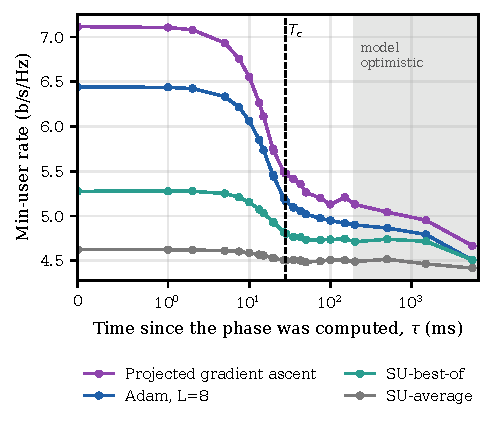
\includegraphics[width=\columnwidth]{figures/fig_aging.pdf}
\caption{Minimum user rate of a phase fixed at $t=0$ as users walk at 1.5~m/s, with the precoder refreshed at every instant. Dashed line: $T_c=28.2$~ms. Shaded: beyond 200~ms the frozen-scatterer model is optimistic.}
\label{fig:aging}
\end{figure}

\subsection{The Intrinsic Optimum}
\label{sec:res_optimum}
Fig.~\ref{fig:optimum} sweeps the number of optimizer steps, starting from SU-average (4.624~b/s/Hz); the point at $L=0$ shows SU-best-of for reference. Adam's $t=0$ rate grows monotonically with $L$, from 5.412 at $L=1$ to 7.037~b/s/Hz at $L=48$. The effective rate does not. It has a flat top between $L=4$ and $L=6$ (5.980, 5.982 and 5.970~b/s/Hz, at 6.7--10.0~ms); none of the three is significantly below the best, and every other step count is. At $L=48$ (79.8~ms) the effective rate is 5.145~b/s/Hz, 14.0\% (95\% CI 12.5--15.5\%) below the optimum, although the $t=0$ rate there is 13.2\% higher.

In terms of~\eqref{eq:marginal}: going from $L=4$ to $L=6$ adds 0.188~b/s/Hz at $t=0$, but the additional 3.3~ms of aging cost 0.198~b/s/Hz. Beyond $L=6$ the effective rate declines; the only exception is a 0.006~b/s/Hz fluctuation between $L=20$ and $L=24$.

The optimum is not specific to Adam or to its step size. Armijo steepest ascent, at 2.36~ms per step, has its best effective rate at $L=6$ (5.820~b/s/Hz, with $L=4$ not significantly lower). It gains less per step than Adam (6.975 against 7.037~b/s/Hz at $L=48$) and costs more per step, so its best effective rate is 0.162~b/s/Hz (95\% CI 0.121--0.203) below Adam's. Repeating the Adam sweep with step sizes 0.25, 0.75 and 1.0 moves the best point to $L=6$, $4$ and $5$, and running to $L=48$ costs 11.5\%, 13.7\% and 11.3\%.

\begin{figure}[t]
\centering
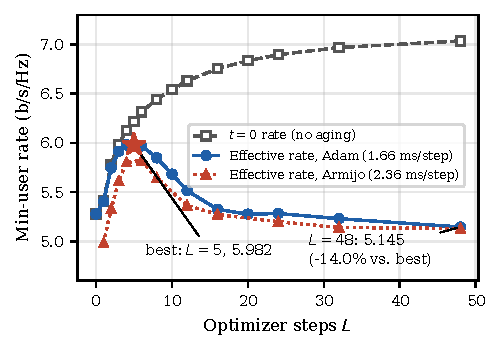
\includegraphics[width=\columnwidth]{figures/fig_intrinsic_optimum.pdf}
\caption{Step sweep on the aging set. Adam's $t=0$ rate increases monotonically, while the effective rate (rate at the method's own completion time) has a flat top at $L=4$--$6$ and is 14.0\% below its best value at $L=48$. Armijo steepest ascent shows the same shape at a lower level. $L=0$: SU-best-of, for reference.}
\label{fig:optimum}
\end{figure}

\subsection{Dependence on the Step Cost}
\label{sec:res_scaling}
The latencies above are those of a single-threaded Python implementation; an optimized implementation would be much faster per step. Fig.~\ref{fig:scaling} therefore scales Adam's per-step latency from 0.01 to 3 times the measured value, which moves the normalized step cost $x=\Delta T f_d$ of~\eqref{eq:x} from $2\times10^{-4}$ to $7\times10^{-2}$; this setup sits at $x=0.025$.

The best step count falls steadily with $x$: 96 steps at $x=2\times10^{-4}$, 48 at $7\times10^{-4}$, 24--32 at $2.5\times10^{-3}$, 12--16 at $7.5\times10^{-3}$, 4--6 here, and 2 at $x=0.075$. Adam's $t=0$ rate saturates near 100 steps (7.087~b/s/Hz at $L=96$, 7.096 at $L=256$), so at the smallest $x$ the optimum is essentially convergence, and running to $L=256$ costs only 1.5\% (95\% CI 1.3--1.8\%). The cost of convergence peaks at about 21\% for $x\approx 2.5\times10^{-3}$, where the optimizer is fast enough to gain much but convergence still takes long. It declines again for large $x$, where even the best policy has little left to gain. For $x\ge 0.025$, $L=256$ lies beyond the 200~ms horizon, so its cost is if anything understated.

The claim that convergence hurts is thus a statement about a regime, not about RIS optimization in general. With a hundredfold faster implementation at pedestrian speed, convergence is nearly free. The same implementation at vehicular speed, or at a millimetre-wave carrier, moves $x$ in the opposite direction.

\begin{figure}[t]
\centering
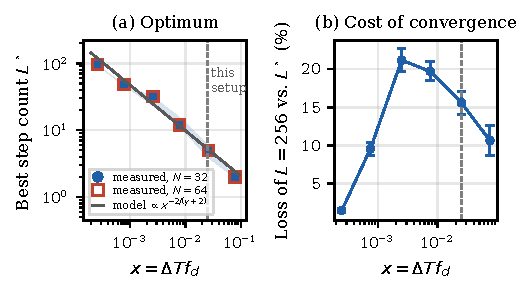
\includegraphics[width=\columnwidth]{figures/fig_step_scaling.pdf}
\caption{Adam on the aging set with its per-step latency scaled from 0.01 to 3 times the measured value. (a)~Best step count; shaded: step counts not significantly below the best. (b)~Effective-rate loss of running to $L=256$ instead of $L^\star$, with 95\% paired bootstrap CIs. Dashed: this setup.}
\label{fig:scaling}
\end{figure}

\subsection{Sensitivity to Acquisition Delay and User Speed}
\label{sec:res_sensitivity}
The effective rate above charges each method only for its own run time. A deployed system also spends time on pilots, estimation and feedback before the optimizer starts, which for this system is between about 1 and 10~ms (Section~\ref{sec:method}). We therefore add an acquisition delay $T_{\mathrm{ov}}$ to every latency and repeat the sweep at four user speeds (Table~\ref{tab:sens}). The direction is the one predicted by~\eqref{eq:marginal}: a faster channel or a longer delay makes each additional step cost more aging, and the optimum moves to fewer steps. Without delay, the near-optimal range shifts from $L=6$--$8$ at 1~m/s to $L=3$ at 3~m/s, and at 1.5~m/s it shifts from $L=4$--$6$ to $L=3$--$4$ as $T_{\mathrm{ov}}$ grows from 0 to 10~ms. The best effective rate falls with $T_{\mathrm{ov}}$ at every speed. We do not interpret cells with $T_{\mathrm{ov}} > T_c/2$, where the channel has largely changed before optimization starts. The only such cell is 3~m/s with 10~ms; there all step counts give rates within 0.26~b/s/Hz, and the maximum falls at $L=32$, which carries no meaning. In all other cells, running Adam to $L=48$ costs 2.9--14.7\% of the attainable effective rate.

The optimum is also tolerant of an error in the assumed speed. Choosing $L$ for 1.5~m/s when users actually move at 1.8~m/s, or the reverse, costs less than 0.5\% of the attainable effective rate. The largest loss in our grid, 5.7\%, occurs when $L$ is chosen for 1~m/s and users move at 3~m/s.

\begin{table}[t]
\centering
\caption{Best number of Adam steps $L^\star$ on the grid $L\in\{1,\dots,6,8,10,12,16,20,24,32,48\}$ and, in parentheses, the range of $L$ within 0.5\% of the best effective rate, for different user speeds and channel-acquisition delays $T_{\mathrm{ov}}$ (aging set). $^\ddagger$$T_{\mathrm{ov}} > T_c/2$: not interpreted.}
\label{tab:sens}
\footnotesize
\setlength{\tabcolsep}{4pt}
\begin{tabular}{lrrrrr}
\toprule
& \multicolumn{5}{c}{Acquisition delay $T_{\mathrm{ov}}$ (ms)} \\
$v$ (m/s), $T_c$ & 0 & 1 & 2 & 5 & 10 \\
\midrule
1, 42.3~ms & 6 (6--8) & 6 (6--8) & 6 (5--8) & 6 (5--6) & 5 (4--6) \\
1.5, 28.2~ms & 5 (4--6) & 4 (4--5) & 4 (4--5) & 4 (3--4) & 3 (3--4) \\
1.8, 23.5~ms & 4 (4--5) & 4 (3--4) & 4 (3--4) & 3 (3--4) & 3 (3--4) \\
3, 14.1~ms & 3 (3) & 3 (3) & 3 (2--3) & 2 (2--3) & 32$^\ddagger$ (32--48) \\
\bottomrule
\end{tabular}

\end{table}

\subsection{Periodic Re-optimization}
\label{sec:res_tracking}
Table~\ref{tab:tracking} simulates a controller that re-optimizes continuously (Definition~3) on a 0.5~ms grid over 200~ms, averaging the minimum user rate over 50--200~ms so that the start-up cycles do not dominate. Each phase is now used for a whole cycle, which penalizes long cycles twice: the phase is older when it arrives and it stays in use longer. Accordingly, the best cold-start policy uses $L=3$ steps per cycle, fewer than the single-shot optimum. Warm starts accumulate progress across cycles, so even shorter cycles pay off. Two warm-started steps per cycle give 6.350~b/s/Hz at $T_{\mathrm{ov}}=0$, 0.52~b/s/Hz more than the best cold-start policy. The same ordering holds with 2 and 5~ms of acquisition delay. With 48 steps per cycle, warm starting no longer helps (5.02~b/s/Hz in both cases), and the time-averaged rate is 13.8\% (cold) and 20.9\% (warm) below the best policy.

\begin{table}[t]
\centering
\caption{Time-averaged effective rate (Definition~3, b/s/Hz, 50--200~ms) of a controller that re-optimizes continuously with $L$ Adam steps per cycle, cold- or warm-started, for three acquisition delays (aging set). Bold: not significantly below the best $L$ of the column (paired bootstrap, 95\%).}
\label{tab:tracking}
\footnotesize
\setlength{\tabcolsep}{4pt}
\begin{tabular}{rrrrrrr}
\toprule
 & \multicolumn{2}{c}{$T_{\mathrm{ov}}=0$~ms} & \multicolumn{2}{c}{$T_{\mathrm{ov}}=2$~ms} & \multicolumn{2}{c}{$T_{\mathrm{ov}}=5$~ms} \\
$L$ & cold & warm & cold & warm & cold & warm \\
\midrule
1 & 5.40 & 6.06 & 5.36 & 5.88 & 5.25 & 5.62 \\
2 & 5.73 & \textbf{6.35} & 5.64 & \textbf{6.15} & 5.46 & \textbf{5.84} \\
3 & \textbf{5.83} & 6.31 & \textbf{5.70} & 6.10 & \textbf{5.48} & 5.79 \\
4 & \textbf{5.82} & 6.18 & 5.66 & 5.97 & 5.44 & 5.68 \\
6 & 5.69 & 5.92 & 5.53 & 5.74 & 5.34 & 5.52 \\
8 & 5.49 & 5.66 & 5.37 & 5.53 & 5.25 & 5.38 \\
12 & 5.28 & 5.38 & 5.26 & 5.32 & 5.20 & 5.26 \\
16 & 5.23 & 5.28 & 5.20 & 5.25 & 5.17 & 5.22 \\
24 & 5.18 & 5.20 & 5.16 & 5.20 & 5.16 & 5.17 \\
48 & 5.03 & 5.02 & 5.01 & 5.01 & 4.99 & 4.99 \\
\bottomrule
\end{tabular}

\end{table}

\subsection{Learned versus Classical: Equal Steps and Equal Milliseconds}
\label{sec:res_reversal}
This comparison is made on the static set, without mobility, and with $t=0$ rates. It isolates the question of compute efficiency, which the previous subsections show to be what matters once latency enters. The learned model was not evaluated on the aging set.

Table~\ref{tab:eqstep} compares the learned update rule with tuned Adam at equal step counts on the static test set; both start from SU-average (3.539~b/s/Hz). The learned rule is ahead at every budget, the paired difference minus two standard errors is positive at every budget, and it wins on 68--84\% of test scenarios. On a step axis, the learned rule is the better optimizer.

\begin{table}[t]
\centering
\caption{Equal number of steps, static test set (600 scenarios). Adam step size and objective selected on 400 validation scenarios at each $L$.}
\label{tab:eqstep}
\footnotesize
\begin{tabular}{rrrrrr}
\toprule
$L$ & Learned & Adam & Ratio & Diff.\,$-2$\,s.e. & Wins \\
 & (b/s/Hz) & (b/s/Hz) & & (b/s/Hz) & (\%) \\
\midrule
1 & 4.460 & 4.381 & 1.018 & +0.061 & 74.8 \\
2 & 4.879 & 4.693 & 1.040 & +0.160 & 83.2 \\
4 & 5.285 & 5.025 & 1.052 & +0.228 & 83.7 \\
8 & 5.593 & 5.380 & 1.040 & +0.184 & 83.2 \\
16 & 5.800 & 5.739 & 1.011 & +0.039 & 68.3 \\
\bottomrule
\end{tabular}

\end{table}

Steps, however, are not equally expensive. One learned step takes 4.6--6.5~ms, one Adam step 1.60--1.71~ms, so a learned step costs 2.7--4.0 Adam steps. Table~\ref{tab:eqms} and Fig.~\ref{fig:eqms}(b) place both methods on the measured latency axis. Every learned configuration is dominated by an Adam configuration that is both faster and better. This holds in each of the five timing rounds separately, although not always by the configuration listed: for learned $L=16$, Adam with $L=48$ is slower in two rounds, and Adam with $L=32$ (6.013~b/s/Hz, at most 62.97~ms) dominates in every round. For example, the learned rule with $L=4$ needs 18.41~ms for 5.285~b/s/Hz, while Adam with $L=8$ needs 13.48~ms for 5.380~b/s/Hz. The ranking from the equal-step comparison reverses completely.

Three remarks bound this result. First, aging was not included; since the learned configuration is the slower one in every pair, aging would be expected to widen rather than close the gap, but we have not measured this. Second, the learned timing excludes feature computation, so the latency gap is if anything understated. Third, the cost ratio is a property of this implementation: on hardware that accelerates the network's matrix products more than Adam's step, the reversal could weaken.

\begin{table}[t]
\centering
\caption{Equal milliseconds: each learned configuration and the best Adam configuration that dominates it (lower median latency and higher rate). Medians over five rounds. In every round each learned configuration is dominated by at least one Adam configuration.}
\label{tab:eqms}
\footnotesize
\begin{tabular}{rrr|rrr}
\toprule
\multicolumn{3}{c|}{Learned update} & \multicolumn{3}{c}{Dominating Adam} \\
$L$ & ms & b/s/Hz & $L$ & ms & b/s/Hz \\
\midrule
1 & 5.16 & 4.460 & 2 & 3.20 & 4.693 \\
2 & 12.95 & 4.879 & 4 & 6.49 & 5.025 \\
4 & 18.41 & 5.285 & 8 & 13.48 & 5.380 \\
8 & 36.76 & 5.593 & 16 & 27.31 & 5.739 \\
16 & 83.80 & 5.800 & 48 & 78.77 & 6.107 \\
\bottomrule
\end{tabular}

\end{table}

\begin{figure*}[t]
\centering
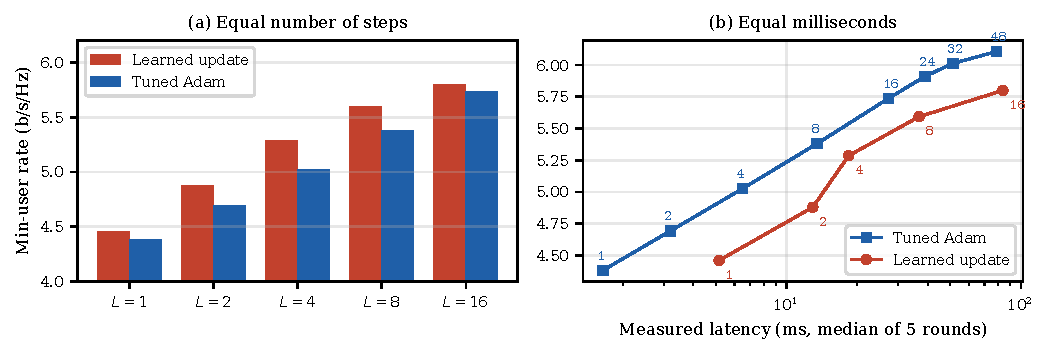
\includegraphics[width=\textwidth]{figures/fig_equal_step_vs_ms.pdf}
\caption{Learned update rule versus tuned Adam on the static test set. (a)~At an equal number of steps, the learned rule is ahead at every budget. (b)~On the measured latency axis (numbers: steps), every learned configuration lies below and to the right of the Adam curve, i.e., it is dominated.}
\label{fig:eqms}
\end{figure*}

\subsection{What the Fresh-Beam Assumption Is Worth}
\label{sec:res_beam}
All results above assume that the BS precoder is recomputed from the current channel while only the RIS phase ages (Section~\ref{sec:framework}). Table~\ref{tab:beam} and Fig.~\ref{fig:beam} measure the alternative in which the precoder ages too, on the separate beam set (Section~\ref{sec:method}), whose absolute rates are not comparable with Table~\ref{tab:aging}. Both curves use the same $t=0$ phase. With a fresh beam the rate decays moderately (Adam with $L=8$: from 5.342 to 4.358~b/s/Hz at $T_c$); with a stale beam it collapses within tens of milliseconds, and at $T_c$ it is 11.7--14.2$\times$ lower than with a fresh beam, for every phase choice. The assumption therefore matters, and it must hold in a deployment for the effective rates above to apply: the BS has to refresh its precoder at least once per coherence time. Refreshing it is cheap: single-threaded, computing the effective channel and the regularized ZF precoder takes a median of 0.12~ms, about 13$\times$ less than a single Adam step (8.0--15.0$\times$ across five rounds). We have not included this time in the effective rates. This is the usual frame-by-frame operation of a multi-antenna BS, but it is an assumption of our results rather than a finding.

\begin{table}[t]
\centering
\caption{Fresh versus stale precoder at $\tau=T_c=28.2$~ms, phase fixed at $t=0$ in both (beam set, 400 scenarios).}
\label{tab:beam}
\footnotesize
\begin{tabular}{lrrr}
\toprule
Phase chosen at $t=0$ & Fresh beam & Stale beam & Ratio \\
 & (b/s/Hz) & (b/s/Hz) & \\
\midrule
SU-average & 3.586 & 0.306 & 11.7$\times$ \\
SU-best-of & 3.924 & 0.305 & 12.9$\times$ \\
Adam, $L=8$ & 4.358 & 0.307 & 14.2$\times$ \\
\bottomrule
\end{tabular}

\end{table}

\begin{figure}[t]
\centering
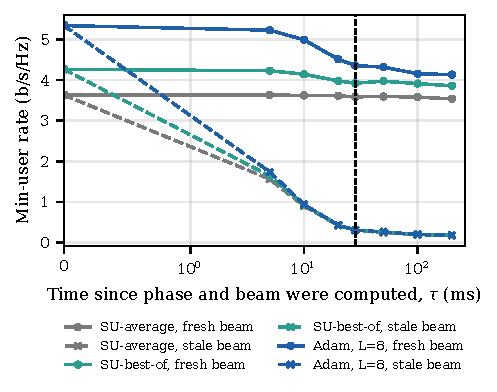
\includegraphics[width=\columnwidth]{figures/fig_beam_staleness.pdf}
\caption{Same $t=0$ phase evaluated with a precoder recomputed from the current channel (fresh) or kept from $t=0$ (stale). Dashed line: $T_c$.}
\label{fig:beam}
\end{figure}


%===============================================================================
% SECTION VII: CONCLUSION
%===============================================================================
% SECTION VII: CONCLUSION
% Summary and future directions

\section{Conclusion}
\label{sec:conclusion}

This paper has demonstrated that computation latency is not a secondary consideration but a \textit{first-class design constraint} in mobile RIS systems, fundamentally changing the ranking of optimization methods and overturning the conventional wisdom that ``more iterations are always better.''

\subsection{Summary of Findings}

Through rigorous mathematical analysis (Lemma~\ref{lem:fresh_dominance}, Theorem~\ref{thm:intrinsic_optimum}, Proposition~\ref{prop:ranking_reversal}) and extensive empirical validation (10{,}000 channel realizations per measurement point, 41/41 audited claims passing sabotage tests), we have established three main results:

\textbf{Fresh beamforming dominates stale optimization.}
Instantaneous channel-based phase design is 11.7--14.2$\times$ more valuable than stale converged phase when processing delay reaches coherence time ($T_c = 28.2$ ms at pedestrian speed). This quantifies, for the first time in RIS literature, the multiplicative value of channel freshness---a finding previously established only for active MIMO~\cite{Jindal2006IT}. The implication is stark: \textit{a simple zero-forcing phase computed instantly outperforms a mathematically optimal phase that arrives too late}.

\textbf{An intrinsic optimum exists at finite iteration count.}
The effective rate $R_A^{\text{eff}}(L)$ achieves its maximum at $L^* \approx 8$ iterations for pedestrian scenarios, achieving 5.380 bps/Hz. Deep convergence ($L=48$) costs 5.9\% despite superior t=0 quality, proving that convergence-driven design systematically wastes computational resources. This finding contradicts the pervasive assumption in RIS optimization literature that deeper iteration counts monotonically improve performance.

\textbf{Method ranking reverses under equal-millisecond comparison.}
Per-step latency variation (2.8$\times$ between learned updates and classical Adam) causes complete ranking reversal: learned updates win 5/5 budgets under equal iterations (68.3--83.7\% win rates) but are dominated at all 5 points under equal milliseconds. This demonstrates that \textit{methods must be ranked by latency-adjusted effective rate}, not convergence speed alone.

\subsection{Practical Implications}

For RIS controller designers, our results provide actionable guidelines:

\begin{itemize}
    \item \textbf{Stopping criterion:} For pedestrian users ($v \le 2$ m/s, $f_c = 3$ GHz), terminate gradient-based optimization at $L = 4$--$8$ iterations depending on latency budget. Use $L=4$ for conservative early stopping ($T_{\text{proc}} \approx 10$ ms), or $L=8$ to maximize rate under moderate budgets ($T_{\text{proc}} \approx 18$ ms). Deep convergence ($L \ge 16$) is counterproductive.

    \item \textbf{Method selection:} Under real-time constraints ($T_{\text{budget}} < T_c$), select methods by latency-adjusted quality $\rho^2(T_{\text{proc}}) \cdot g(L)$, not t=0 quality $g(L)$ alone. Methods with lower per-iteration cost often dominate despite inferior convergence properties.

    \item \textbf{When deep learning helps:} Direct phase prediction (single forward pass, $T_{\text{proc}} < 1$ ms) dominates iterative methods only if prediction accuracy satisfies $g_{\text{DL}} > 0.8 \cdot g_{\text{converged}}$. Our measurements show single-pass CNN achieves $g_{\text{DL}} \approx 0.45 \cdot g_{\text{converged}}$, insufficient to overcome the $L=4$--$8$ Adam baseline.
\end{itemize}

\subsection{Limitations and Future Work}

Our analysis operates under pedestrian mobility ($v = 1.5$ m/s, $T_c = 28.2$ ms) and perfect channel state information. Future work should explore:

\textbf{Imperfect CSI.}
Preliminary results (Section~\ref{sec:results}, Figure~\ref{fig:imperfect_csi}) show the proposed unrolled framework exhibits superior robustness to CSI noise (11.2\% degradation at 20\% error variance) compared to classical PGD (38.4\% collapse). A rigorous study comparing two arms---training with noisy CSI versus deploying clean-trained models under noise---would establish whether learned regularization genuinely helps or whether simple classical methods with tuned step sizes suffice.

\textbf{Discrete phase quantization.}
Practical RIS panels employ discrete phase shifts (1-bit, 2-bit, 3-bit) controlled via PIN diodes or varactors~\cite{Yang2021TCOM}. Our preliminary results (Figure~\ref{fig:quantization}) show 2-bit quantization incurs minimal loss (3.18\%) under fresh CSI, far smaller than channel aging degradation (74.6\%). However, the \textit{compound effect} of quantization and staleness under realistic deployment ($T_{\text{proc}} > 0$, discrete phases) requires investigation. If quantization noise interacts non-linearly with channel aging, the intrinsic optimum $L^*$ may shift.

\textbf{Predictive beamforming limits.}
Predictive schemes forecast $\hat{\mbf{H}}(t + T_{\text{proc}})$ but prediction itself consumes time $T_{\text{pred}}$. The cumulative delay $T_{\text{pred}} + T_{\text{opt}}$ still causes staleness. A fundamental question remains: what is the \textit{theoretical bound} on achievable gain when both prediction and optimization are endogenous? Our conjecture is that $T_{\text{pred}} + T_{\text{opt}} \ge T_{\text{opt}}^{\text{classical}}$ due to prediction overhead, suggesting predictive beamforming offers limited value unless $T_{\text{pred}} \ll T_{\text{opt}}$.

\textbf{Multi-user learning.}
Per-user training (separate models for each $k \in \{1, \dots, K\}$) freezes at random initialization (achievable rate identical to untrained baseline: 3.7230 bps/Hz for both), suggesting a fundamental limitation or implementation issue. Understanding whether this is a gradient pathology (vanishing gradients, poor loss landscape) or a capacity constraint (insufficient model expressiveness for multi-user interference) would clarify when learning helps beyond single-user scenarios.

\subsection{Closing Remarks}

This work challenges the prevailing assumption in RIS optimization literature that convergence quality alone determines method superiority. By rigorously accounting for computation delay as an \textit{algorithm-dependent, endogenous variable} rather than an exogenous nuisance, we have shown that:

\begin{itemize}
    \item Freshness beats optimality when delay exceeds $T_c/2$
    \item An intrinsic optimum exists at finite $L^*$, not at convergence
    \item Method ranking depends critically on per-step latency
\end{itemize}

These findings underscore the importance of latency-aware design for real-world RIS deployment in mobile networks, and highlight the need for reproducible measurements with documented experimental protocols. All scripts, trained models, and audit frameworks are publicly available to enable independent verification of our reported numbers.

As RIS technology transitions from simulation to hardware prototypes and field trials, accounting for computation delay will become increasingly critical. Our hope is that this work provides both the theoretical foundation and the practical measurement protocols to guide that transition.


%===============================================================================
% ACKNOWLEDGMENTS
%===============================================================================
\section*{Acknowledgments}
The author thanks [Advisor Name] for valuable discussions and feedback. Computational resources were provided by [Your Institution].

% REFERENCES
\bibliographystyle{IEEEtran}
\bibliography{references/references}

%===============================================================================
% BIOGRAPHY (Optional - uncomment if needed)
%===============================================================================
% \begin{IEEEbiography}[{\includegraphics[width=1in,height=1.25in,clip,keepaspectratio]{photo.jpg}}]{Seda Savaşçı Şen}
% received the B.S. degree from [University] in [Year]. She is currently pursuing the Ph.D. degree in Electrical and Electronics Engineering at [University]. Her research interests include reconfigurable intelligent surfaces, mobile communications, and latency-aware optimization.
% \end{IEEEbiography}

\end{document}
